\pdfoutput=1
 
\documentclass{l4proj}
\usepackage[usenames,dvipsnames]{xcolor}
\usepackage{enumitem}
\usepackage{hyperref}
\usepackage{titlesec}
\usepackage{listings}
\titlespacing{\subsubsection}{0pt}{6pt}{6pt}
\definecolor{properBlue}{HTML}{336699}
\hypersetup{
    colorlinks,
    citecolor=properBlue,
    filecolor=properBlue,
    linkcolor=properBlue,
    urlcolor=properBlue
}
 
\begin{document}
\title{Package Recommendation Engine}
\author{Keir Alexander Smith}
\date{March 15, 2015}
\maketitle
 
\begin{abstract}
This paper covers the construction of a basic recommendation engine for operating system packages, specifically for use with the DNF package manager. The tool should allow users to discover useful packages through an easy to use command line interface.
\end{abstract}
 
%\educationalconsent
\tableofcontents

\lstset{ %
language=Python,              % choose the language of the code
basicstyle=\scriptsize,     % the size of the fonts that are used for the code
%basicstyle=\tiny,     % the size of the fonts that are used for the code
numbers=left,               % where to put the line-numbers
%numberstyle=\tiny,    % the size of the fonts that are used for the line-numbers
numberstyle=\scriptsize,    % the size of the fonts that are used for the line-numbers
numbersep=10pt,             % how far the line-numbers are from the code
frame=trBL,                 % adds a frame around the code
%tabsize=2,                  % sets default tabsize to 2 spaces
captionpos=b,               % sets the caption-position to bottom
breaklines=true,            % sets automatic line breaking
breakatwhitespace=false,    % sets if automatic breaks should only happen at whitespace
showstringspaces=false,     % Don't show underscores as space characters
frameround=fttt
}
 
%%%%%%%%%%%%%%%%%%
%                %
%  INTRODUCTION  %
%                %
%%%%%%%%%%%%%%%%%%
 
\chapter{Introduction}
\pagenumbering{arabic}
 
\section{Problem overview}
In a modern operating system there exist many packages for end users to install and this collection grows every day\cite{debpopcon}. Finding useful packages to install can be a laborious task, often involving the use of online search to track down the package the user has been looking for, if it exists. In a series of informal interviews, one users quoted: \emph{"Sometimes, I'll use Google as it has a more intelligent understanding of what I might be looking for and can recommend packages that aren't exact searches"}.\\
Furthermore there exists little support for installing packages commonly installed concurrently. Debian offers a 'recommended' field in a package's meta data which the author can set manually. For example when a user who has vim\footnote{A well used and long standing text editor for Linux. See http://www.vim.org/about.php} installed then installs JDK\footnote{Java Development Kit. See http://www.oracle.com/technetwork/java/javase/overview/index.html}, the user may not be aware of the existence of a Java plugin for vim which could be extremely useful.

\section{Motivation}
Package management is an interesting and very useful tool for many users, however the basic implementation has been static for many years. With the addition of a package recommendation system, we could see a decrease in users having to use search engines to look for packages they should be able to discover easily on command line or local GUI interaction.\\
Furthermore if this project can be used as a base to look into package grouping and weighting of relationships between packages. Hopefully this could lead to some very interesting use cases and provide a lot of data for analysis.
 
\section{Aims}
This project aims to attempt to address the issues discussed above. Primarily the problem of finding new packages by offering a powerful recommendation system for users to discover packages.\\
Consider a user on a Linux machine, looking for any new useful developer tools to help their work flow. Using an internet search engine returns a massive set of results with various levels of relevance, this project aims to supply that user with a command line interface where they can ask for a recommendation based on package of their choice. In an example scenario our user asks for a recommendation based off of the Java Development Kit package and is returned with a list of useful debugging tools and plugins which they weren't aware of previously.

\section{Report outline}
This report will be structured as the following:
\begin{itemize}
\item Background - A look into the research undertaken for this project in order to design the system
\item Design - A collection of design documents and details of how the system will be implemented and operated by the end user
\item Evaluation - Discussion of how useful the system is as well as how well designed it may be
\item Conclusion - A final chapter to wrap up the report as a whole and discuss future potential work
\end{itemize}
 
%%%%%%%%%%%%%%%%
%              %
%  BACKGROUND  %
%              %
%%%%%%%%%%%%%%%%
 
\chapter{Background}
A package manager\footnote{Examples include dpkg for Debian (http://linux.die.net/man/1/dpkg), YUM for Red Hat Linux (http://yum.baseurl.org/) and pacman for Arch Linux (https://www.archlinux.org/pacman/)} allows users to search for, install and update packages containing useful programs. For many years Unix has relied on package managers to allow easy management of tools and underlying applications. However in recent times, as package numbers increase and the ease of search engines becomes more prominent, searching using a command line tool has become less prevalent. Unless a user knows exactly what they want, often times they will resort to a internet search engine to find new packages. One user in an informal interview quoted the following: \emph{"I generally know the name of the program I want, so `pacman -Ss name` to find the package name"}

\section{Modern Graphical Package Managers}
\begin{figure}
\centerline{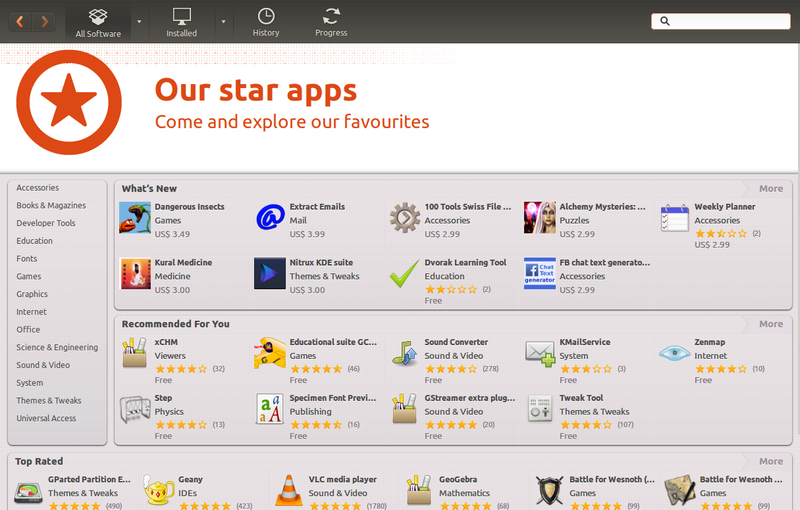
\includegraphics[scale=0.5]{images/ubuntu_software.png}}
\caption{Ubuntu Software Center}
\end{figure}
A more modern solution to this problem is the use of Graphical User Interfaces (GUIs)\footnote{For example the Ubuntu Software Center shown in Figure 2.1.} to abstract the annoyance of searching on command line away from the user. However this requires that the user is running a system with graphical output, a luxury which is often not found when running Virtual Machines (VMs) or using Secure Shell (SSH).

\section{NuGet Concierge}
NuGet\cite{nuget} is a package manager for Microsoft's .net framework. It's seen large growth since its introduction and has expanded greatly to cover many tools. In 2013 NuGet introduced a new service called Concierge\cite{concierge} which allowed users to upload their project metadata and get recommended packages to use back from the service.\\
Concierge works by giving each package a popularity score and then giving each package pair a bi-directional pairing weighting, shown in Figure 2.1. It then expects a project.conf file from the user, which it parses and uses the list of required packages to recommend a set of packages from the graph.\\
Concierge was build by a group of Microsoft interns in order to see what they could do with the growing user and package base. However it seems that, as of writing, the project has been abandoned, with the last commit to their GitHub\footnote{https://github.com/NuGet/Concierge} repository in 2013.
\begin{figure}
\centerline{\fbox{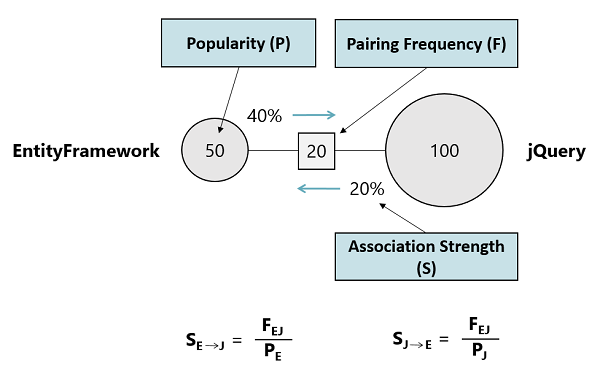
\includegraphics[scale=1]{images/nuget_graph.png}}}
\caption{NuGet Concierge's internal structure}
\end{figure}

\section{DNF}
My project aims to supply similar recommendation functionality to users of DNF\footnote{http://fedoraproject.org/wiki/Features/DNF}, Fedora 21's new package manager. DNF allows plugins to be easily added by simply dropping a Python file into the plugins directory. This allows DNF to be extended easily with little hardship from the user. Building in functionality into DNF is exactly the behaviour this project aims to provide to the end user.\\ 

%%%%%%%%%%%%
%          %
%  DESIGN  %
%          %
%%%%%%%%%%%%
 
\chapter{Design}
This system comes in two parts, a client side plugin for DNF which the user installs by dropping a single Python script into the correct directory. Also a server side database to store user's installed packages, anonymously, and provide data for recommendations. See Figure 3.1\\
Each of these components will be discussed in their own sections.
\begin{figure}
\centerline{\fbox{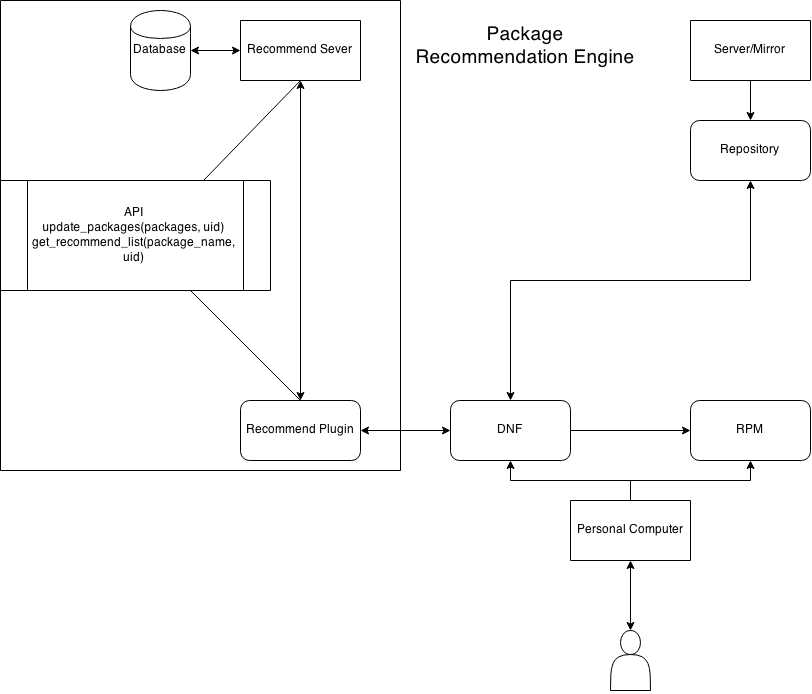
\includegraphics[scale=0.6]{images/packagerecommend.png}}}
\caption{System Diagram}
\end{figure}

\section{Recommend Plugin}
In the choice between DNF and dpkg/apt, DNF was chosen due to its excellent plugin support over the alternative.\\
The Recommend plugin has two key features:
\begin{itemize}
\item Request recommendation from server
\item Upload user's installed packages anonymously
\end{itemize}
Both functions require a connection to the back end database, a connection over the internet is assumed.\\
The plugin needed to be easy to use, otherwise the user will resort to a simple web search. With this in mind it was designed with two clear commands. See Figure 3.2\\
\begin{figure}
\centerline{\fbox{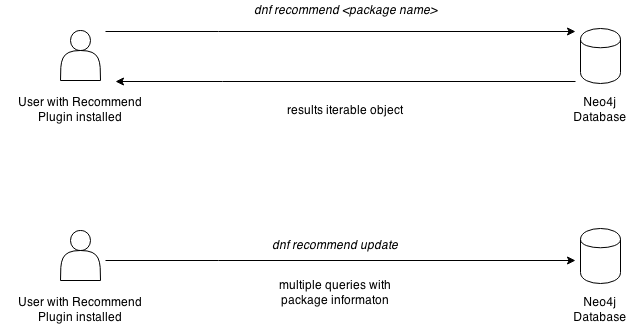
\includegraphics[scale=0.7]{images/recommend_api.png}}}
\caption{Diagram showing the exchanges between the server and client}
\end{figure}


\section{Database}
The project requires a back end data storage module. Immediately a database comes to mind for a long term, concurrent access method of storing and returning large volumes of data. Below the various potential choices of database are discussed.

\subsection{Selection}
Neo4j was selected as the database of choice for this project. There are several key reasons for this:\\
\begin{center}
\begin{tabular}{|c|c|}
\hline
\textbf{mySQL} & \textbf{Neo4j}\\
\hline
Path finding is difficult & Path finding optimised\\
\hline
Many to Many relations expensive & Many to Many relations light weight\\
\hline
Expensive joins & Rapid pattern matching\\
\hline
Designed to work on one machine & Designed to scale across machines\\
\hline
\end{tabular}
\end{center}
With these point in mind, it seemed the logical choice to make use of a graph database like Neo4j for the purposes of the system.

\subsection{Internal Structure}
Internally the structure of the graph can be seen in Figure 3.3
\begin{figure}
\fbox{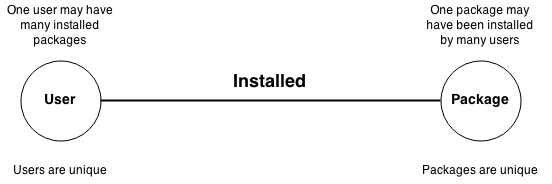
\includegraphics[scale=0.9]{images/recommend_graph.png}}
\caption{Diagram showing the internal structure of the database}
\end{figure} 
Users are stored as unique nodes within the graph, each with a unique user ID attached to them. This allows us to generate their user id when they first upload their package information, the ID generated is entirely random so the user remained anonymous.\\
Packages are all uniquely stored with their name as their unique identifier, this means package versions are not considered when making recommendations.\\

\subsection{Keeping Up to Date}
As users install and un-install packages the user must update the database with their new state. If the database is not kept up to date it may run into problems making recommendations of deprecated packages or not recommending new packages.\\
Users may not willing go out their way to update regularly, therefore the following methods were considered to allow users to keep up to date:\\
\begin{itemize}
\item Every time the user installs/un-installs a package, automatically update
\item On DNF initialisation prompt the user to update
\item Update automatically in set periods
\end{itemize}

\subsection{Security}
Security was a serious consideration during design, since malicious users could easily tamper with our data. The resulting decision was to ignore security for the scope of this project, however points to be considered will be listed below.\\
\begin{itemize}
\item Users could create many fake users with potentially malicious implications
\item Users could run arbitrary cypher scripts on the database server
\item Users could upload users with fake package information
\item Users could potentially overload server capacity via a Denial of Service\footnote{See http://searchsoftwarequality.techtarget.com/definition/denial-of-service} attack.
\end{itemize}

%%%%%%%%%%%%%%%%%%%%
%                  %
%  IMPLEMENTATION  %
%                  %
%%%%%%%%%%%%%%%%%%%%
 
\chapter{Implementation}
In regards to development environment, all work took place using a GitHub repository with all the Python scripts kept up to date there. Locally the Recommend plugin was kept in the Git repository folder which was then sym linked to the DNF plugin folder. This enabled work and change tracking to take place without disturbing work flow to test the plugin.\\
With the design settled, work began with a 'Wizard of Oz'\cite{wizofoz} style mock up, where the user could use the command line interface as if the system were complete, however anything they go back was simply place holder.

\section{First Pass Mock UI}
For this initial development two features needed to be implemented. A command to push a list of installed packages to server and another to request a recommendation from the server.\\
DNF allows a developer to hook into its core functionality by extending classes, which allows new commands to be written and functionality added in a single Python script. Figure 4.1 and 4.2 shows two classes extending DNF plugin and command classes respectively.
\begin{figure}
\lstset{caption={Recommend Class},label=codeRecClass}
\lstinputlisting[lastline=7]{code/recommend.py}
\end{figure}
\begin{figure}
\lstset{caption={Recommend Command Class},label=codeRecCommClass}
\lstinputlisting[firstline=9]{code/recommend.py}
\end{figure}

\section{Back End Implementation}
Now that some form of client side had been written, the back end could be implemented. This turned into a simple case of installing and running a Neo4j instance on a local machine to test scripts.\\
The initial script written, shown in listing 4.3, read a list of packages from a text file in the format which DNF dumps them and then created each on the database and tied them to a user with a fake ID.\\
With that was in place, scripts, shown in listing 4.5, to find sets of recommendations between packages can be written and tested.\\
See Figures 4.1 through 4.3 for graphic examples of how the Neo4j stores user and package information.\\
\begin{figure}
\fbox{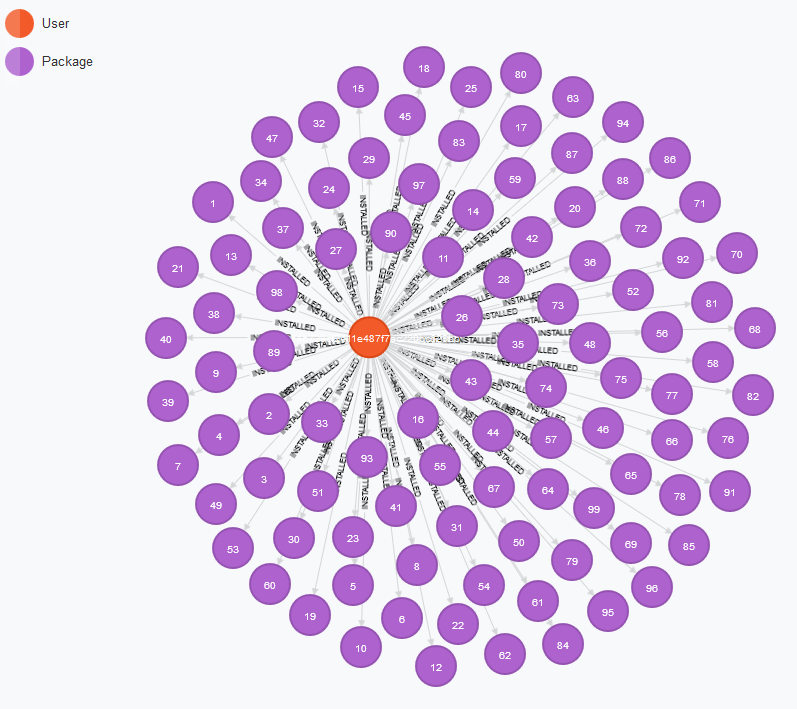
\includegraphics[scale=0.8]{images/recommend_graph_user.png}}
\caption{Example of a single real user}
\end{figure}
\begin{figure}
\fbox{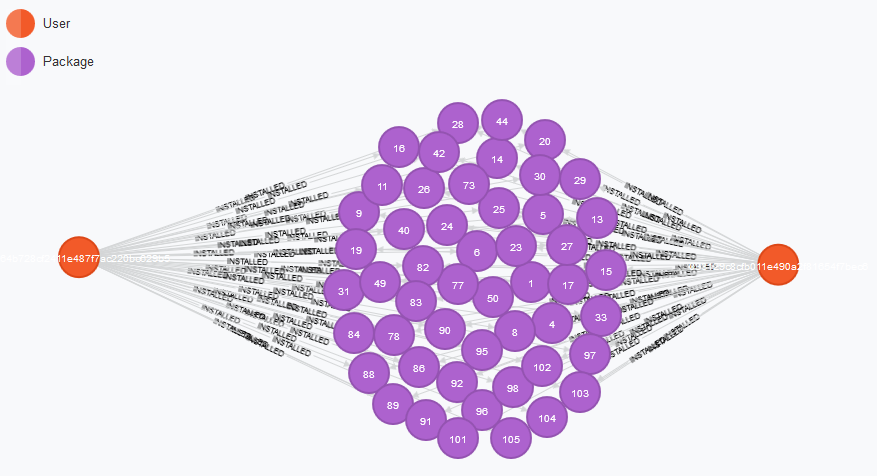
\includegraphics[scale=0.75]{images/recommend_graph_packages.png}}
\caption{Example of two real users sharing packages}
\end{figure}
\begin{figure}
\fbox{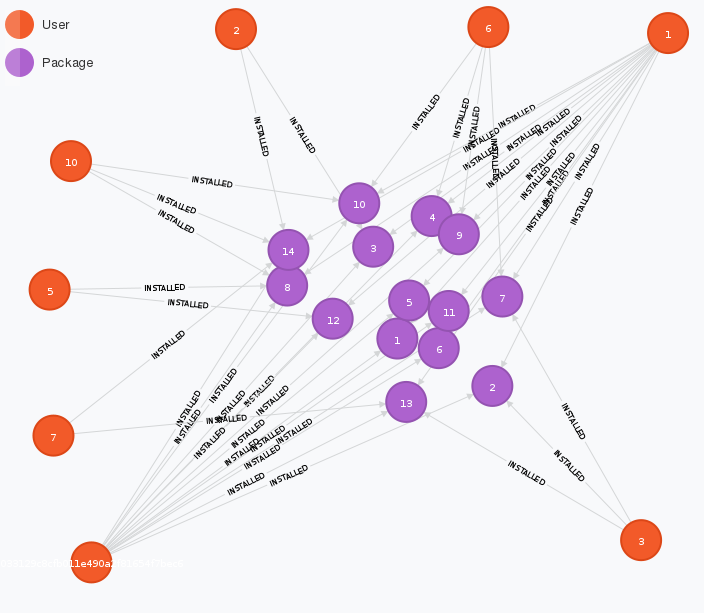
\includegraphics[scale=0.9]{images/recommend_graph_sharing.png}}
\caption{Example of 8 mock users sharing various packages}
\end{figure}

\section{Bringing it together}
With the client side UI already written and tested, it was a simple case of changing a constant defining the server address to the operational database which was running on local host.

\section{Testing}
In order to test this system, two scripts were written in Python to fill the database with both real and mock data. Several small Cypher scripts were also written to test that the database was working internally.\\
Listings 4.3 and 4.4 show the Python scripts for entering data.\\
\begin{figure}
\lstset{caption={Fills the graph with real data},label=codeGraphReal}
\lstinputlisting[firstline=3]{code/graph.py}
\end{figure}
\begin{figure}
\lstset{caption={Fills the graph with mock data},label=codeGraphMock}
\lstinputlisting[firstline=4]{code/graph_filler.py}
\end{figure}
Using a database prepared with data from either of these scripts, a series of cypher queries were run to ensure relationships, users and packages were being correctly translated. See Listings 4.5 for these test queries.
\begin{figure}
\lstset{caption={A collection of test Cypher queries},label=queryCyperTest}
\lstinputlisting[firstline=1]{code/cypher_test.txt}
\end{figure}
 
%%%%%%%%%%%%%%%%
%              %
%  EVALUATION  %
%              %
%%%%%%%%%%%%%%%%
 
\chapter{Evaluation}
All evaluation was based on a series of short, informal interviews with 5 users.\\
Majority of users found the concept appealing and were interested to use the system. One user in particular could relate well to the problem.\\
In using the system, no users had trouble with the user interface, but majority commented on the lack of help and the formatting of the output. One user said \emph{"It's concise, but it just needs the format tidied up so it is easier on the eyes to read"}.\\
All users asked how reliable the recommendations were, as they seemed unsatisfied with the results they were given. One user commented specifically on how his input to the recommend command didn't seem to make any difference to the output of the recommendations.\\
Four of the five users said they wouldn't use it themselves, with the last user saying they would use the system, but only if it included more specific filter options.\\
Over all the evaluation has shown the system will need work before being used in a live environment, however it does show promise.
 
%%%%%%%%%%%%%%%%
%              %
%  CONCLUSION  %
%              %
%%%%%%%%%%%%%%%%
 
\chapter{Conclusion}

\section{Summary}
To conclude the report, the system as a whole was written using a series of small Python scripts, with the main script being the DNF plugin. A neo4j instance is running on a remote server allowing users to use the system live.\\
The final system met the minimum requirements. The user is able to upload their installed packages to the database and then ask for a recommendation.\\
The idea is well received, with users overall agreeing it is an interesting avenue to explore. However many who tried the application were weary of the limited scope of getting recommendations and most users stated they would only use the system if it had finer grain recommendation control.

\section{Future Work}
There exists a lot of scope for this project to expand. This section will discuss two interesting areas for potential future work.

\subsection{Package Groups}
As a potential future addition, commonly installed package groups could be identified on the back end, which would be pushed forward to end users, allowing them to quickly install a complete set of tools.\\
An example of this would be web developers, who commonly install at least the three main browsers\footnote{Google Chrome, Mozilla Firefox and Safari} and any debugging/developer tools associated with them.\footnote{For example Firebug}\\
This kind of powerful inferencing can be done using a graph database made to look for groups like this. If it's possible to then analyse the group and identify what it is, this would give users a lot of power when installing packages clusters.  

\subsection{Weighted Relationships} 
Weighted relationships is something which NUGET Concierge used to make its recommendations. It's a one directional value assigned between two package nodes to determine how likely it is that one is installed on the same system with the other.\\
At its core, it's very simple, however we could go lengths to make this weighting more meaningful, perhaps through the use of labels or special cases we can identify when best to include packages in a recommendation. For example it may be the case that package X is usually only installed when package Y is installed and Z isn't. A weighted relationship would not identify this as it would only recommend the most common. By tagging the relationships we can ensure the correct recommendation is made to the user.

\section{Lessons Learned}
A recommendation system is a powerful tool, however it suffers from Metcalfe's law, where in a network is proportionally valuable to the square of the number of nodes. With a small number of users the recommendations have very low value, more than not being complete gibberish. However as you scale the system up, these recommendations become more valuable.\\

%%%%%%%%%%%%%%%%
%              %
%  APPENDICES  %
%              %
%%%%%%%%%%%%%%%%
 
 
%%%%%%%%%%%%%%%%%%%
%                 %
%  BIBLIOGRAPHY   %
%                 %
%%%%%%%%%%%%%%%%%%%
 
\bibliographystyle{plain}
\bibliography{bib}
\end{document}